\documentclass{article}

  % packages
    % basic stuff for rendering math
    \usepackage[letterpaper, top=1in, bottom=1in, left=1in, right=1in]{geometry}
    \usepackage[utf8]{inputenc}
    \usepackage[english]{babel}
    \usepackage{amsmath} 
    \usepackage{amssymb}

    % extra math symbols and utilities
    \usepackage{mathtools}        % for extra stuff like \coloneqq
    \usepackage{mathrsfs}         % for extra stuff like \mathsrc{}
    \usepackage{centernot}        % for the centernot arrow 
    \usepackage{bm}               % for better boldsymbol/mathbf 
    \usepackage{enumitem}         % better control over enumerate, itemize
    \usepackage{hyperref}         % for hypertext linking
    \usepackage{xr-hyper}
    \usepackage{fancyvrb}          % for better verbatim environments
    \usepackage{newverbs}         % for texttt{}
    \usepackage{xcolor}           % for colored text 
    \usepackage{listings}         % to include code
    \usepackage{lstautogobble}    % helper package for code
    \usepackage{parcolumns}       % for side by side columns for two column code
    

    % page layout
    \usepackage{fancyhdr}         % for headers and footers 
    \usepackage{lastpage}         % to include last page number in footer 
    \usepackage{parskip}          % for no indentation and space between paragraphs    
    \usepackage[T1]{fontenc}      % to include \textbackslash
    \usepackage{footnote}
    \usepackage{etoolbox}

    % for custom environments
    \usepackage{tcolorbox}        % for better colored boxes in custom environments
    \tcbuselibrary{breakable}     % to allow tcolorboxes to break across pages

    % figures
    \usepackage{pgfplots}
    \pgfplotsset{compat=1.18}
    \usepackage{float}            % for [H] figure placement
    \usepackage{tikz}
    \usepackage{tikz-cd}
    \usepackage{circuitikz}
    \usetikzlibrary{arrows}
    \usetikzlibrary{positioning}
    \usetikzlibrary{calc}
    \usepackage{graphicx}
    \usepackage{algorithmic}
    \usepackage{caption} 
    \usepackage{subcaption}
    \captionsetup{font=small}

    % for tabular stuff 
    \usepackage{dcolumn}

    \usepackage[nottoc]{tocbibind}
    \pdfsuppresswarningpagegroup=1
    \hfuzz=5.002pt                % ignore overfull hbox badness warnings below this limit

  % New and replaced operators
    \DeclareMathOperator{\Tr}{Tr}
    \DeclareMathOperator{\Sym}{Sym}
    \DeclareMathOperator{\Span}{span}
    \DeclareMathOperator{\std}{std}
    \DeclareMathOperator{\Cov}{Cov}
    \DeclareMathOperator{\Var}{Var}
    \DeclareMathOperator{\Corr}{Corr}
    \DeclareMathOperator{\pos}{pos}
    \DeclareMathOperator*{\argmin}{\arg\!\min}
    \DeclareMathOperator*{\argmax}{\arg\!\max}
    \newcommand{\ket}[1]{\ensuremath{\left|#1\right\rangle}}
    \newcommand{\bra}[1]{\ensuremath{\left\langle#1\right|}}
    \newcommand{\braket}[2]{\langle #1 | #2 \rangle}
    \newcommand{\qed}{\hfill$\blacksquare$}     % I like QED squares to be black

  % Custom Environments
    \newtcolorbox[auto counter, number within=section]{question}[1][]
    {
      colframe = orange!25,
      colback  = orange!10,
      coltitle = orange!20!black,  
      breakable, 
      title = \textbf{Question \thetcbcounter ~(#1)}
    }

    \newtcolorbox[auto counter, number within=section]{exercise}[1][]
    {
      colframe = teal!25,
      colback  = teal!10,
      coltitle = teal!20!black,  
      breakable, 
      title = \textbf{Exercise \thetcbcounter ~(#1)}
    }
    \newtcolorbox[auto counter, number within=section]{solution}[1][]
    {
      colframe = violet!25,
      colback  = violet!10,
      coltitle = violet!20!black,  
      breakable, 
      title = \textbf{Solution \thetcbcounter}
    }
    \newtcolorbox[auto counter, number within=section]{lemma}[1][]
    {
      colframe = red!25,
      colback  = red!10,
      coltitle = red!20!black,  
      breakable, 
      title = \textbf{Lemma \thetcbcounter ~(#1)}
    }
    \newtcolorbox[auto counter, number within=section]{theorem}[1][]
    {
      colframe = red!25,
      colback  = red!10,
      coltitle = red!20!black,  
      breakable, 
      title = \textbf{Theorem \thetcbcounter ~(#1)}
    } 
    \newtcolorbox[auto counter, number within=section]{proposition}[1][]
    {
      colframe = red!25,
      colback  = red!10,
      coltitle = red!20!black,  
      breakable, 
      title = \textbf{Proposition \thetcbcounter ~(#1)}
    } 
    \newtcolorbox[auto counter, number within=section]{corollary}[1][]
    {
      colframe = red!25,
      colback  = red!10,
      coltitle = red!20!black,  
      breakable, 
      title = \textbf{Corollary \thetcbcounter ~(#1)}
    } 
    \newtcolorbox[auto counter, number within=section]{proof}[1][]
    {
      colframe = orange!25,
      colback  = orange!10,
      coltitle = orange!20!black,  
      breakable, 
      title = \textbf{Proof. }
    } 
    \newtcolorbox[auto counter, number within=section]{definition}[1][]
    {
      colframe = yellow!25,
      colback  = yellow!10,
      coltitle = yellow!20!black,  
      breakable, 
      title = \textbf{Definition \thetcbcounter ~(#1)}
    } 
    \newtcolorbox[auto counter, number within=section]{example}[1][]
    {
      colframe = blue!25,
      colback  = blue!10,
      coltitle = blue!20!black,  
      breakable, 
      title = \textbf{Example \thetcbcounter ~(#1)}
    } 
    \newtcolorbox[auto counter, number within=section]{code}[1][]
    {
      colframe = green!25,
      colback  = green!10,
      coltitle = green!20!black,  
      breakable, 
      title = \textbf{Code \thetcbcounter ~(#1)}
    } 
    \newtcolorbox[auto counter, number within=section]{algo}[1][]
    {
      colframe = green!25,
      colback  = green!10,
      coltitle = green!20!black,  
      breakable, 
      title = \textbf{Algorithm \thetcbcounter ~(#1)}
    } 

    \definecolor{dkgreen}{rgb}{0,0.6,0}
    \definecolor{gray}{rgb}{0.5,0.5,0.5}
    \definecolor{mauve}{rgb}{0.58,0,0.82}
    \definecolor{darkblue}{rgb}{0,0,139}
    \definecolor{lightgray}{gray}{0.93}
    \renewcommand{\algorithmiccomment}[1]{\hfill$\triangleright$\textcolor{blue}{#1}}

    % default options for listings (for code)
    \lstset{
      autogobble,
      frame=ltbr,
      language=Python,
      aboveskip=3mm,
      belowskip=3mm,
      showstringspaces=false,
      columns=fullflexible,
      keepspaces=true,
      basicstyle={\small\ttfamily},
      numbers=left,
      firstnumber=1,                        % start line number at 1
      numberstyle=\tiny\color{gray},
      keywordstyle=\color{blue},
      commentstyle=\color{dkgreen},
      stringstyle=\color{mauve},
      backgroundcolor=\color{lightgray}, 
      breaklines=true,                      % break lines
      breakatwhitespace=true,
      tabsize=3, 
      xleftmargin=2em, 
      framexleftmargin=1.5em, 
      stepnumber=1
    }

  % Page style
    \pagestyle{fancy}
    \fancyhead[L]{}
    \fancyhead[C]{Muchang Bahng}
    \fancyhead[R]{Spring 2025} 
    \fancyfoot[C]{\thepage / \pageref{LastPage}}
    \renewcommand{\footrulewidth}{0.4pt}          % the footer line should be 0.4pt wide
    \renewcommand{\thispagestyle}[1]{}  % needed to include headers in title page

  % external documents 
  %  \externaldocument[place-]{../Machine_Learning/paper}[../Machine_Learning/paper.pdf] 

\begin{document}

\title{C}
\author{Muchang Bahng}
\date{Spring 2025}

\maketitle
\tableofcontents
\pagebreak

\section{Implementations of Memory Structures in C} 

  \subsection{Arrays}

  \subsection{Strings}

  \subsection{Structs}

  \subsection{Functions}

  \subsection{Input Output}
    
    We have standard in, standard out, and standard error. 


\section{TBD} 

  With this structure in mind and knowing the size of some primitive types, we can now focus on how declaring them works in the backend. 

  \begin{definition}[Declaration, Initialization]
    Assigning a value to a variable is a two step process, which is often not distinguished in high level languages like Python. 
    \begin{enumerate}
      \item You must first \textbf{initialize} the variable by setting aside the correct number of bytes in memory. 
      \item You must then \textbf{assign} that variable to be some actual value. 
    \end{enumerate}
    The two step process is often called declaration. 
  \end{definition}

  This is the reason why C is statically, or strongly, typed. In order to set aside some memory for a variable, you must know how big that variable will be, which you know by its type. This makes sense. We can first demonstrate how to both initialize and declare a variable. 

  \begin{figure}[H]
    \centering 
    \noindent\begin{minipage}{.5\textwidth}
    \begin{lstlisting}[]{Code}
      int main() {
        // declaring 
        int x = 4;   
        printf("%p\n", &x); 
        
        // initializing and assigning
        int y; 
        printf("%p\n", &y); 
        y = 3; 
        printf("%p\n", &y); 

        return 0; 
      }
    \end{lstlisting}
    \end{minipage}
    \hfill
    \begin{minipage}{.49\textwidth}
    \begin{lstlisting}[]{Output}
      0x16d37ee68
      0x16d37ee64
      0x16d37ee64 
      .
      .
      .
      .
      .
      .
      .
      .
      .
      .
    \end{lstlisting}
    \end{minipage}
    \caption{How to declare variables in C. As you can see, by initializing \texttt{y}, the memory address is already assigned and it doesn't change when you assign it. The address is only shown to be 9 hex digits long, but it is actually 16 hex digits long and simply 0 padded on the left. } 
    \label{fig:declaring_initializing_variables}
  \end{figure}

  One question that may come to mind is, what is the value of the variable if you just initialize it? After all the value at that address that is initialized must be either $0$s or $1$s. Let's find out. 

  \begin{figure}[H]
    \centering 
    \noindent\begin{minipage}{.5\textwidth}
    \begin{lstlisting}[]{Code}
      int main() { 
        int y; 
        printf("%d\n", y); 
        y = 3; 
        printf("%d\n", y); 

        return 0; 
      }
    \end{lstlisting}
    \end{minipage}
    \hfill
    \begin{minipage}{.49\textwidth}
    \begin{lstlisting}[]{Output}
      6298576 
      3
      .
      .
      .
      .
      .
      .
    \end{lstlisting}
    \end{minipage}
    \caption{The value of an uninitialized variable is some random number. } 
    \label{fig:uninitialized_variable}
  \end{figure}

  It may be interesting to see how this random unititialized value is generated. It is simply the value that was stored in that memory address before, and it is not cleared when you initialize it, so you should not use this as a uniform random number generator. 


  \subsection{Debugging and Object Dumping} 

    Talk about gdb, lldb, objdump, etc. These are debugging tools that allow you to parse your code line by line. However, to actually see the C code, you must compile it with the debugging flag. This adds a little bit of overhead memory to the binary, but not a lot. 

  \subsection{Type Casting}


  \subsection{Pointers}

    We have learned how to declare/initialize a variable, which frees up some space in the memory and possibly assigns a value to it. One great trait of C is that we can also store the memory address of a variable in another variable called a pointer. You access both the memory and the value at that memory with this pointer variable. 

    \begin{definition}[Pointer Variable]
      A \textbf{pointer} variable/type is a variable that stores the memory address of another variable. 
      \begin{enumerate}
        \item You can declare a pointer in the same way that you declare a variable, but you must add a asterisk in front of the variable name. 
        \item The size of this variable is the size of the memory address, which is 8 bytes in a 64-bit architecture. 
        \item To get the value of the variable that the pointer points to, called \textbf{dereferencing}, you simply put a asterisk in front of the pointer. This is similar to how you put a ampersand in front of a variable to get its memory address. 
      \end{enumerate}

      \begin{figure}[H]
        \centering 
        \noindent\begin{minipage}{.5\textwidth}
        \begin{lstlisting}[]{Code}
          int main() { 
            // declare an integer 
            int x = 4; 
            printf("x = %d\n", x); 
            printf("&x = %p\n", &x); 

            // declare pointer 
            int *p = &x; 
            printf("p = %p\n", p); 
            printf("*p = %d\n", *p); 

            // initialize pointer 
            int *q; 
            q = &x; 
            printf("q = %p\n", q); 
            printf("*q = %d\n", *q); 
            return 0; 
          }
          
        \end{lstlisting}
        \end{minipage}
        \hfill
        \begin{minipage}{.49\textwidth}
        \begin{lstlisting}[]{Output}
          x = 4
          &x = 0x16d49ae68
          p = 0x16d49ae68
          *p = 4
          q = 0x16d49ae68
          *q = 4
          .
          .
          .
          .
          .
          .
          .
          .
          .
          .
          .
          .
        \end{lstlisting}
        \end{minipage}
        \caption{} 
        \label{fig:pointer_variable}
      \end{figure}
    \end{definition}

    Since the size of addresses are predetermined by the architecture, it may not seem like we need to know the underlying data type of what it points to, so why do we need to write strongly type the underlying data type? Remember that to do pointer arithmetic, you need to know how large the underlying data type is so that you can know how many bytes to move when traversing down an array. 

    One of the reasons why pointers are so valuable is that they allow you to pass by reference, which is a way to change the value of a variable in a function. 

    \subsubsection{Call by Value vs Call by Reference}

      \begin{definition}[Call by Value]
        
      \end{definition}

      \begin{definition}[Call by Reference]
        
      \end{definition}
    
    \subsubsection{Pointer Errors}

      Just like for regular variables, you may be curious on the value of an unassigned pointer. Let's take a look. 

      \begin{example}[Uninitialized Pointers]
      \begin{figure}[H]
        \centering 
        \noindent\begin{minipage}{.5\textwidth}
        \begin{lstlisting}[]{Code}
          int main() { 
            int x = 4; 
            int *p; 
            printf("p = %p\n", p); 
            printf("*p = %x\n", *p); 

            return 0; 
          }
        \end{lstlisting}
        \end{minipage}
        \hfill
        \begin{minipage}{.49\textwidth}
        \begin{lstlisting}[]{Output}
          p = 0x10249ff20
          *p = d100c3ff
          .
          .
          .
          .
          .
          .
        \end{lstlisting}
        \end{minipage}
        \caption{The value of an uninitialized pointer is some random address and at a random address it would be some random byte. } 
        \label{fig:uninitialized_pointer}
      \end{figure}
      \end{example}

      This is clearly not good, especially since the program compiles correctly and runs without any errors. This kind of pointer that hasn't been initialized is called a wild pointer. 

      \begin{definition}[Wild Pointer]
        A \textbf{wild pointer} is a pointer that has not been initialized to a known value. 
      \end{definition}

      To fix this, we must always initialize a pointer to a known value. This may come at a disadvantage, since now we can't reap the benefits of initializing first and assigning later. A nice compromise is to initialize the pointer to a null pointer. 

      \begin{definition}[Null Pointer]
        A \textbf{null pointer} is a pointer that has been initialized to a known value, which is the address 0x0. You can set the type of the pointer and then initialize it to \texttt{NULL}. 
      \begin{figure}[H]
        \centering 
        \noindent\begin{minipage}{.5\textwidth}
        \begin{lstlisting}[]{Code}
          int main() { 
            int *p = NULL; 
            printf("p = %p\n", p); 
            
            // the code below gives seg fault
            /* printf("*p = %d\n", *p); */

            int x = 4; 
            p = &x; 
            printf("p = %p\n", p); 
            printf("*p = %d\n", *p);
            return 0; 
          }
        \end{lstlisting}
        \end{minipage}
        \hfill
        \begin{minipage}{.49\textwidth}
        \begin{lstlisting}[]{Output}
          p = 0x0
          p = 0x16da72e5c
          *p = 4
          .
          .
          .
          .
          .
          .
          .
          .
          .
          .
        \end{lstlisting}
        \end{minipage}
        \caption{Initializing a null pointer. It is a good practice to initialize a pointer to a null value. } 
        \label{fig:null_pointer}
      \end{figure}
      \end{definition}

      Therefore, the null pointer allows you to set the type of the underlying data type, but the actual address will be 0x0. You cannot dereference a null pointer, and doing so will give you a segmentation fault. There may be times when you do not even know the data type of the pointer, and for this you can use the void pointer, which now doesn't know the type of the variable that it points to but it does allocate address. 

      \begin{definition}[Void Pointer]
        A \textbf{void pointer} is a pointer that does not know the type of the variable that it points to. We can initialize it by simply setting the underlying type to be void. This initializes the address, which should always be 8 bytes, but trying to access the value of the variable is not possible. 
        \begin{figure}[H]
          \centering 
          \noindent\begin{minipage}{.5\textwidth}
          \begin{lstlisting}[]{Code}
            int main() { 
              void *p; 
              printf("p = %p\n", p); 
              int x = 4; 
              p = &x; 
              printf("%d", *((int*)p));
              return 0; 
            }
          \end{lstlisting}
          \end{minipage}
          \hfill
          \begin{minipage}{.49\textwidth}
          \begin{lstlisting}[]{Output}
            p = 0x102553f54
            4 
            .
            .
            .
            .
            .
            .
          \end{lstlisting}
          \end{minipage}
          \caption{Initialize a void pointer and then use typecasting to access the value of the variable that it points to. } 
          \label{fig:initialize_void_pointer}
        \end{figure}
      \end{definition}

  \subsection{Pointer Arithmetic} 

    With pointers out of the way, we can talk about how arrays are stored in memory. 

    \begin{definition}[Array]
      A C array is a collection of elements of the same type, which are stored in contiguous memory locations. You can initialize and declare arrays in many ways, and access their elements with the index, e.g. \texttt{arr[i]}.
      \begin{enumerate}
        \item You declare an array of some constant number of elements $n$ with the elements themselves. 
          \begin{lstlisting} 
            int arr[5] = {1, 2, 3, 4, 5}; 
          \end{lstlisting}
        \item You declare an array with out its size $n$ and simply assign them. Then $n$ is automatically determined. 
          \begin{lstlisting} 
            int arr[] = {1, 2, 3, 4, 5}; 
          \end{lstlisting}
        \item You initialize an array of some constant size $c$, and then you assign each element of the array. 
          \begin{lstlisting} 
            int arr[5]; 
            for (int i = 0; i < 5; i++) {
              arr[i] = i + 1; 
            }
          \end{lstlisting}
      \end{enumerate}
      Unfortunately, C does not provide a built-in way to get the size of the array (like \texttt{len} in Python), so we must keep track of the size of the array ourselves. Furthermore, the address of the array is the address of where it begins at, i.e. the address of the first element. 
    \end{definition}

    You can literally see that the elements of the array are contiguous in memory by iterating through each element and printing out its address. 

    \begin{figure}[H]
      \centering 
      \noindent\begin{minipage}{.5\textwidth}
      \begin{lstlisting}[]{Code}
        int main(void) {
          // initialize array 
          int arr[5]; 
          for (int val = 1; val < 6; val++) {
            arr[val-1] = val * val;
          }

          int* p = &arr[0]; 
          for (int i = 0; i < 5; i++) {
            printf("Value at position %d : %d\n", i, arr[i]); 
            printf("Address at position %d : %p\n", i, p + i); 
          }

          return 0; 
        }        
      \end{lstlisting}
      \end{minipage}
      \hfill
      \begin{minipage}{.49\textwidth}
      \begin{lstlisting}[]{Output}
        Value at position 0 : 1
        Address at position 0 : 0x7ffd8636b0d0
        Value at position 1 : 4
        Address at position 1 : 0x7ffd8636b0d4
        Value at position 2 : 9
        Address at position 2 : 0x7ffd8636b0d8
        Value at position 3 : 16
        Address at position 3 : 0x7ffd8636b0dc
        Value at position 4 : 25
        Address at position 4 : 0x7ffd8636b0e0
        .
        .
        .
        .
        .
        .
        .
      \end{lstlisting}
      \end{minipage}
      \caption{Ints are 4 bytes long, so the address of the next element is 4 bytes away from the previous element, making this a contiguous array.} 
      \label{fig:contiguous_array}
    \end{figure}

    The most familiar implementation of an array is a string in C. 

    \begin{definition}[String]
      A string is an array of characters, which is terminated by a null character \texttt{\textbackslash 0}. You can initialize them in two ways: 
      \begin{enumerate}
        \item You can declare a string with the characters themselves, which you must make sure to end with the null character. 
          \begin{lstlisting} 
            char str[6] = {'H', 'e', 'l', 'l', 'o', '\0'}; 
          \end{lstlisting}
        \item You can declare them with double quotes, which automatically adds the null character. 
          \begin{lstlisting} 
            char str[] = "Hello"; 
          \end{lstlisting}
      \end{enumerate}
      Note that for whatever string we initialize, the size of the array is the number of characters plus 1. 
    \end{definition}

    To access elements of an array, you simply use the index of the element, e.g. \texttt{arr[i]}, but in the backend, this is implemented with \textit{pointer arithmetic}. 

    \begin{definition}[Pointer Arithmetic]
      Pointer arithmetic is the arithmetic of pointers, which is done by adding or subtracting an integer to a pointer. 
      \begin{enumerate}
        \item If you add an integer $n$ to a pointer $p$, e.g. \texttt{p + n}, then the new pointer will point to the $n$th element after the current element, with the next element being \texttt{sizeof(type)} bytes away from the pervious element. 
        \item If you subtract an integer $n$ from a pointer, then the pointer will point to the $n$th element before the current element. 
      \end{enumerate}
      This is why you can access the elements of an array with the index, since the index is simply the number of elements away from the first element.
    \end{definition}

    \begin{example}[Pointer Arithmetic with Arrays of Ints and Chars]
      Ints have a size of 4 bytes and chars 1 byte. You can see that using pointer arithmetic, the addresses of the elements of ints increment by 4 and those of the char array increment by 1. 
      \noindent\begin{minipage}{.5\textwidth}
      \begin{lstlisting}[]{Code}
        int main() { 
          int integers[3] = {1, 2, 3}; 
          char characters[3] = {'a', 'b', 'c'};
          int *p = &integers[0]; 
          char *q = &characters[0];
          
          printf("Array of Integers\n"); 
          for (int i = 0; i < 3; i++) { 
            printf("%p\n", integers+i); }

          printf("Array of Characters\n"); 
          for (int i = 0; i < 3; i++) { 
            printf("%p\n", characters+i); }
          return 0; 
        }
      \end{lstlisting}
      \end{minipage}
      \hfill
      \begin{minipage}{.49\textwidth}
      \begin{lstlisting}[]{Output}
        Array of Integers
        0x16d39ee58
        0x16d39ee5c
        0x16d39ee60
        .
        Array of Characters
        0x16d39ee50
        0x16d39ee51
        0x16d39ee52
        .
        .
        .
        .
        .
        .
      \end{lstlisting}
      \end{minipage}
    \end{example}

    Therefore, we can think of accessing the elements of an array as simply pointer arithmetic. 

    \begin{theorem}[Bracket Notation is Pointer Arithmetic]
      The bracket notation is simply pointer arithmetic in the backend. 
      \begin{figure}[H]
        \centering 
        \noindent\begin{minipage}{.5\textwidth}
        \begin{lstlisting}[]{Code}
          int main() { 
            int arr[3] = {1, 2, 3}; 
            int *p = &arr[0]; 

            for (int i = 0; i < 3; i++) { 
              printf("%d\n", arr[i]); 
              printf("%d\n", *(p+i)); 
            }
            return 0; 
          }
        \end{lstlisting}
        \end{minipage}
        \hfill
        \begin{minipage}{.49\textwidth}
        \begin{lstlisting}[]{Output}
          1
          1
          2
          2
          3
          3
          .
          .
          .
          .
        \end{lstlisting}
        \end{minipage}
        \caption{Accessing the elements of the list using both ways is indeed the same. } 
        \label{fig:bracket_pointer_arthimetic}
      \end{figure}
    \end{theorem}
   
  \subsection{Global, Stack, and Heap Memory}

    Everything in a program is stored in memory, variables, functions, and even the code itself. However, we will find out that they are stored in different parts of the memory. When a program runs, its application memory consists of four parts, as visualized in the Figure \ref{fig:memory_layout}. 
    \begin{enumerate} 
      \item The \textbf{code} is where the code text is stored. 
      \item The \textbf{global memory} is where all the global variables are stored. 
      \item The \textbf{stack} is where all of the functions and local variables are stored. 
      \item The \textbf{heap} is variable and can expand to as much as the RAM on the current system. We can specifically store whatever variables we want in the heap.
    \end{enumerate}

    We provide a visual of these four parts first, and we will go into them later. 
    \begin{figure}[H]
      \centering 
      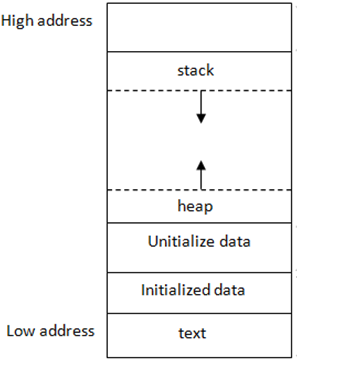
\includegraphics[scale=0.6]{img/memory_layout.png}
      \caption{The four parts of memory in a C program.} 
      \label{fig:memory_layout} 
    \end{figure}

    \begin{definition}[Code Memory]
      This is where the code text is stored. It is read-only and is not modifiable.
    \end{definition}

    In high level languages, we always talk about local and global scope. That is, variables defined within functions have a local scope in the sense that anything we modify in the local scope does not affect the global scope. We can now understand what this actually means by examining the backend.  The global scope variables are stored in the global memory, and all local variables (and functions) are stored in the stack. 


    \begin{definition}[Global Memory]
      This is where all the global variables are stored. 
    \end{definition}

    \begin{definition}[Stack Memory]
      This is where all of the functions and local variables are stored. As we will see later, the compiler will always run the main function, which must exist in your file. By the main function is a function itself, and therefore it has its own local scope. 

      Then, when you initialize any functions or local variables within those functions (which will be the majority of your code), all these will be stored in the stack, which is an literally an implementation of the stack data structure. It is LIFO, and the first thing that goes in is the \texttt{main} function and its local variables, which is referred to as the \textbf{stack frame}. You can't free memory in the stack unless its in the top of the stack. 
    \end{definition}

    To see what happens in the stack, we can go through an example. 

    \begin{example}[Going through the Stack]
      Say that you have the following code: 

      \begin{lstlisting} 
        int total; 
        int Square(int x) {
          return x*x; 
        }
        int SquareOfSum(int x, int y) {
          int z = Square(x + y); 
          return z; 
        }
        int main() { 
          int a = 4, b = 8;              
          total = SquareOfSum(a, b); 
          printf("output = %d", total); 
          return 0; 
        }
      \end{lstlisting}
      
      The memory allocation of this program will run as such: 
      \begin{enumerate} 
        \item The \texttt{total} variable is initialized and is put into global memory. 
        \item \texttt{main} is called. It is put into the stack. 
        \item The local variables \texttt{a=4} and \texttt{b=8} are initialized and are put into the stack. 
        \item The \texttt{SquareOfSum} function is called and put into the stack. 
        \item The input local variables \texttt{x=4}, \texttt{y=8}, \texttt{z} are initialized and put into the stack. 
        \item \texttt{x + y=12} is computed and put into the stack. 
        \item The \texttt{Square} function is called and put into the stack. 
        \item The \texttt{x=12} local variable of \texttt{Square} is initialized and put into the stack. 
        \item The CPU computes \texttt{x*x=144} and returns the output. The \texttt{Square} function is removed from the stack. 
        \item We assign \texttt{z=144} and \texttt{SquareOfSum} returns it. Now \texttt{SquareOfSum} is removed from the stack. 
        \item \texttt{total=144} is assigned in the global memory still. 
        \item The \texttt{printf} function is called and put into the stack. 
        \item The \texttt{printf} function prints the output and is removed from the stack. 
        \item The \texttt{main} function returns \texttt{0} and is removed from the stack, ending our application. 
      \end{enumerate}
    \end{example}


    One limitation of the stack is that its total available memory is fixed from the start, ranging from 1MB to 8MB, and so you can't initialize arrays of billions of integers in the stack. It will cause a memory overflow. In fact, the memory of the stack, along with the global and text memory, are assigned at compile time, making it a \textbf{static memory}. 

    Since the stack is really just a very small portion of available memory, the heap comes into rescue, which is the pool of memory available to you in RAM. 

    \begin{definition}[Heap Memory]
      The \textbf{heap memory} (nothing to do with the heap data structure) is a variable length (meaning it can grow at runtime) and \textbf{dynamically allocated} (meaning that we can assign memory addresses during runtime) memory that is limited to your computer's hardware. Unlike simply initializing variables to allocate memory as in the stack, we must use the \textbf{malloc} and \textbf{free} functions in C, and \textbf{new} and \textbf{delete} operations in C++. 
    \end{definition}

    \begin{definition}[malloc]
      
    \end{definition}

    \begin{definition}[free]
      
    \end{definition}

    The stack can store pointer variables that point to the memory address in the heap. So the only way to access variables in the heap is through pointer reference, and the stack provides you that window to access that big pool of heap memory. 


    One warning: if you allocate another address, the previous address does not get deallocated off the memory. 

    \begin{definition}[Memory Leak]
      
    \end{definition}

    On the other hand, if you free an address but have a pointer still pointing to that address, this is also a problem called the dangling pointer. 

    \begin{definition}[Dangling Pointer]
      
    \end{definition}

    At this point, we might be wondering why we need both a stack and a heap. Well the benefits of heaps are clearer since you can dynamically allocate memory, and you don't have the LIFO paradigm that is blocking you from deallocating memory that has been allocated in the beginning of your program. A problem with just having heap is that stacks can be orders of magnitude times faster when allocating/deallocating from it than the heap, and the sequence of function calls is naturally represented as a stack. 

  \subsection{Dynamic Memory Allocation}

    Let's talk about how \texttt{malloc} and \texttt{free} are implemented in C. If you make a for loop and simply print all the addresses that you allocate to. You will find that they can be quite random. After a program makes some calls to malloc and free, the heap memory can becomes fragmented, meaning that there are chunks of free heap space interspersed with chunks of allocated heap space. The heap memory manager typically keeps lists of different ranges of sizes of heap space to enable fast searching for a free extent of a particular size. In addition, it implements one or more policies for choosing among multiple free extents that could be used to satisfy a request.

    The free function may seem odd in that it only expects to receive the address of the heap space to free without needing the size of the heap space to free at that address. That’s because malloc not only allocates the requested memory bytes, but it also allocates a few additional bytes right before the allocated chunk to store a header structure. The header stores metadata about the allocated chunk of heap space, such as the size. As a result, a call to free only needs to pass the address of heap memory to free. The implementation of free can get the size of the memory to free from the header information that is in memory right before the address passed to free.


\end{document}
